\documentclass[12pt]{article}
\usepackage{graphicx}
\usepackage{indentfirst}
\usepackage{polski}
\usepackage{amsmath}
\usepackage{amssymb}
\usepackage{dirtree}
\usepackage{listings}
\usepackage{hyperref}
\usepackage{minted}
\usepackage{xcolor}
\usepackage{subcaption}
\definecolor{LightGray}{gray}{0.9}
\usepackage{tocloft}
\usepackage{hyperref}
\hypersetup{
    colorlinks=true,
    linkcolor=blue
}
\newtheorem{example}{Przykład}

\title{Dokumentacja projektu zespołowego nr 2}
\author{Anna Ćwiklińska, Krystian Gronkowski, Ihor Malyi}
\date{Maj 2023}

\begin{document}
\lstset{basicstyle=\ttfamily, columns=fullflexible, upquote=true}
\renewcommand{\lstlistingname}{Listing}

\maketitle
\newpage
{\hypersetup{hidelinks}
\tableofcontents
}
\newpage
\section{Treść zadania}
Pobrać od użytkownika żądaną dokładność $0<\varepsilon<1$ oraz przedział $[a,b]$, w~którym szukamy pierwiastka równania $$\ln(x^2) - \sin(x) - 2 = 0.$$

Porównać liczbę kroków potrzebnych metodzie siecznych Newtona, by osiągnąć dokładność $\varepsilon$ z~liczbą kroków dla metody bisekcji dla kilku wybranych przedziałów zawierających dokładnie jeden pierwiastek. Znaleźć wszystkie pierwiastki równania z~dokładnością $10^{-8}$.

\section{Teoretyczny opis metod}
\subsection{Metoda siecznych Newtona}
Metoda siecznych Newtona to jedna z~metod numerycznych służących do znajdowania miejsc zerowych funkcji. Metoda ta polega na przybliżaniu pierwiastka równania poprzez konstrukcję linii siecznej przechodzącej przez dwa punkty na wykresie funkcji i~wyznaczeniu jej przecięcia z~osią OX. Następnie punkt ten jest wykorzystywany w~kolejnej iteracji metody, aż do uzyskania dostatecznie dokładnego wyniku.

W~metodzie siecznych Newtona w~każdej iteracji przybliżenie pierwiastka równania jest obliczane jako przecięcie linii siecznej z~osią OX, zdefiniowanej jako:

$$x_{n+1} = x_n - \frac{f(x_n)(x_n-x_{n-1})}{f(x_n)-f(x_{n-1})},\ n\geq1$$

gdzie $x_n$ i~$x_{n-1}$ są kolejnymi przybliżeniami pierwiastka równania, a~$f(x)$ jest funkcją, której pierwiastka szukamy.

\begin{example}
Rozważmy równanie $\ln(x^2) - \sin(x) - 2 = 0$. Chcemy znaleźć pierwiastek tego równania z~dokładnością $\varepsilon = 0.1$.

Zacznijmy od wybrania dwóch początkowych przybliżeń pierwiastka równania, na przykład $x_0 = 2$ i~$x_1 = 3$. Następnie stosujemy wzór metody siecznych Newtona:

$$x_{n+1} = x_n - \frac{f(x_n)(x_n-x_{n-1})}{f(x_n)-f(x_{n-1})},\ n\geq1$$
\begin{enumerate}
    \item Iteracja
    
    Dla $n=0$ mamy:
\begin{align*}
    &f(x_0) = f(2) = -1,523\\
    &f(x_1) = f(3) = 0,0561\\
    &x_{2} = 3 - \frac{0,0561\cdot (3-2)}{0,0561-(-1,523)} \approx 2,9645
\end{align*}
\item Iteracja

Dla $n=1$ mamy:
\begin{align*}
    &f(x_1) = f(3) = 0,0561\\
    &f(x_2) = f(2,9645) = -0,0028\\
    &x_{3} = 2,9645 - \frac{-0,0028\cdot(2,9645-3)}{-0,0028-0,0561} \approx 2,9662
\end{align*}
\end{enumerate}


Obliczamy różnicę między kolejnymi przybliżeniami:
$$|x_{3} - x_{2}| = | 2,9662 - 2,9645| \approx 0,0017$$

Ponieważ wartość ta jest mniejsza niż zadana dokładność $\varepsilon = 0.1$, kończymy obliczenia i~zwracamy ostatnie przybliżenie $x_3 = 2,9662$ jako przybliżenie rozwiązania.
\end{example}

\subsection{Metoda bisekcji}
Dla funkcji ciągłej $f$ określonej na przedziale domkniętym $[a,b]$ oraz spełniającej warunek $f(a) \cdot f(b) < 0$ (czyli funkcja zmienia znak na tym przedziale) możemy znaleźć pierwiastek równania $f(x) = 0$ poprzez wykonanie kroków algorytmu:

\begin{enumerate}
\item Ustawiamy $a_0 = a$, $b_0 = b$, $i = 0$.
\item Obliczamy $c_i = \frac{a_i + b_i}{2}$.
\item Jeśli $f(c_i) = 0$, kończymy obliczenia i zwracamy $c_i$ jako rozwiązanie.
\item Jeśli $f(a_i) \cdot f(c_i) < 0$, ustawiamy $a_{i+1} = a_i$ oraz $b_{i+1} = c_i$.
\item W przeciwnym przypadku, gdy $f(b_i) \cdot f(c_i) < 0$, ustawiamy $a_{i+1} = c_i$ oraz $b_{i+1} = b_i$.
\item Jeśli osiągnięto zadany poziom dokładności (czyli $|b_i - a_i| < \varepsilon$, gdzie $\varepsilon$ to ustalona wartość dokładności), zwracamy $c_i$ jako rozwiązanie.
\item W przeciwnym przypadku, ustawiamy $i = i + 1$ i wracamy do kroku 2.
\end{enumerate}

Algorytm kończy się, gdy zostanie osiągnięty poziom dokładności lub zostanie wykonana maksymalna liczba iteracji. Warto zauważyć, że metoda bisekcji zawsze znajduje pierwiastek równania $f(x) = 0$ na danym przedziale $[a,b]$, pod warunkiem, że funkcja $f$ jest ciągła i zmienia znak na tym przedziale. Metodę bisekcji można jednak stosować tylko wtedy, gdy mamy określony przedział liczbowy, w którym znajduje się dokładnie jeden pierwiastek. W~metodzie tej liczba kroków potrzebnych do uzyskania zadanej dokładności zależy jedynie od początkowego przedziału i wartości $\varepsilon$.

Możemy również zdefiniować błąd oszacowania wartości pierwiastka jako $|c_i - c_{i-1}|$, gdzie $c_i$ to wartość pierwiastka obliczona w $i$-tej iteracji. Błąd ten maleje monotonicznie z każdą kolejną iteracją.


\begin{example}
Dane jest równanie $\ln(x^2) - \sin(x) - 2 = 0$ oraz przedział $[a, b] = [2,3]$.
W celu znalezienia pierwiastka z dokładnością $\varepsilon = 0.1$ zostanie użyta metoda bisekcji.

\begin{enumerate}
\item Iteracja:\\
\begin{align*}
&f(2)=-1.523<0 \quad \text{i} \quad f(3)=0.0561>0\\
&\text{Zatem pierwiastek leży między 2 i 3.}\\
&x_0=\frac{3+2}{2}=2.5\\
&f(x_0)=f(2.5)=\ln(6.25)-\sin(2.5)-2=-0.7659\\
&|f(x_0)|>\varepsilon
\end{align*}
    
    \item Iteracja:\\
\begin{align*}
    &f(2.5)=-0.7659<0 \quad \text{i} \quad f(3)=0.0561>0\\
    &\text{Zatem pierwiastek leży między 2.5 i 3.}\\
    &x_1=\frac{2.5+3}{2}=2.75\\
    &f(x_1)=f(2.75)=\ln(7.5625)-\sin(2.75)-2=-0.3585\\
    &|f(x_1)|>\varepsilon
\end{align*}

    
    \item Iteracja:\\
\begin{align*}
    &f(2.75)=-0.3585<0 \quad \text{i} \quad f(3)=0.0561>0\\
    &\text{Zatem pierwiastek leży między 2.75 i 3.}\\
    &x_2=\frac{2.75+3}{2}=2.875\\
    &f(x_2)=f(2.875)=\ln(8.2656)-\sin(2.875)-2=-0.1513\\
&|f(x_1)|>\varepsilon
\end{align*}
    
    \item Iteracja:\\
\begin{align*}
    &f(2.875)=-0.1513<0 \quad \text{i} \quad f(3)=0.0561>0\\
    &\text{Zatem pierwiastek leży między 2.875 i 3.}\\
    &x_3=\frac{2.875+3}{2}=2.9375\\
    &f(x_3)=f(2.9375)=\ln(8.6289)-\sin(2.9375)-2=-0.0476\\
    &|f(x_3)|<\varepsilon
\end{align*}
\end{enumerate}

Zatem $x \approx 2.9375$
\end{example}
\newpage
\section{Opis programu}
Program został napisany w języku Python3. Składa się on z zestawu plików, używa modułu ABC (Abstract Base Classes) oraz korzysta z biblioteki math.

Celem programu jest porównanie ilości iteracji algorytmów metody bisekcji i metody siecznych Newtona do znalezienia pierwiastka równania $$\ln(x^2) - \sin(x) - 2 = 0$$ na wybranych przedziałach zawierających dokładnie jeden pierwiastek.
\begin{figure}[H]
  \centering
  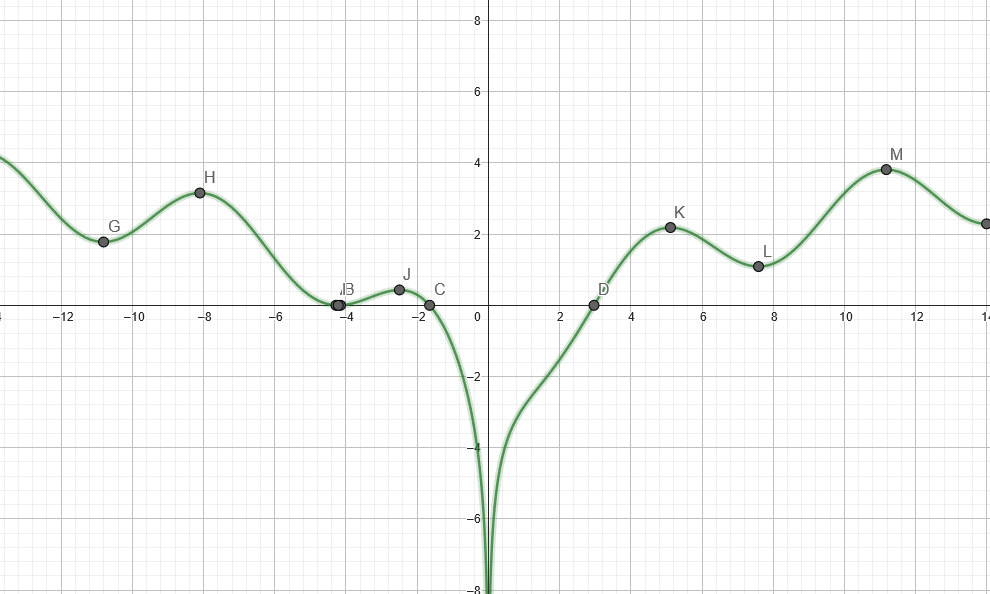
\includegraphics[width=0.9\textwidth]{Firefox_Screenshot_2023-04-28T10-41-17.086Z.png}
  \caption{Wykres funkcji $\ln(x^2) - \sin(x) - 2$ z programu GeoGebra}
  \label{fig:zdjecie1}
\end{figure}
Ponadto, celem programu jest też znalezienie wszystkich pierwiastków powyższego równania z dokładnością $10^{-8}$.
Z wykresu funkcji można odczytać, że rozwiązania równania to:

\begin{itemize}
    \item $A=-4.2812562227602$
    \item $B=-4.1547005187224$
    \item $C=-1.651399905763$
    \item $D=2.9661586753516$
\end{itemize}

\section{Opis algorytmu}
Poniżej znajdują sie opisy algorytmów zaimplementowanych metod numerycznych, które są użyte do szukania pierwiastka z danych wprowadzonych przez użytkownika oraz szukania wszystkich pierwiastków równania.
\subsection{Metoda bisekcji}
\begin{enumerate}
\item Tworzy klasę \verb|Bisection| dziedziczącą po klasie \verb|Method|.
\item W konstruktorze klasy \verb|Bisection| przypisuje wartości przedziału (section), dokładności \verb|e| oraz funkcji (\verb|key|), której wartość zerowa jest poszukiwana.
\item W funkcji \verb|solution|:
\begin{enumerate}
\item Sprawdza, czy przedział zawiera wartość 0. Jeśli tak, wyświetla się komunikat o błędzie i zwraca wartość 0 i krok 0.
\item Sprawdza, czy wartości funkcji na końcach przedziału mają różne znaki. Jeśli nie, wyświetla się komunikat o błędzie i zwraca wartość 0 i krok 0.
\item Ustawia \verb|c| na wartość 1 i krok na 0.
\item Dopóki wartość funkcji w punkcie \verb|c| nie jest równa 0 i różnica między końcami przedziału jest większa niż \verb|e|:
\begin{enumerate}
\item Oblicza \verb|c| jako środek przedziału.
\item Sprawdza, czy wartość funkcji w punkcie \verb|self.section[0]| pomnożona przez wartość funkcji w punkcie \verb|c| jest mniejsza niż 0. Jeśli tak, ustawia wartość \verb|self.section[1]| na \verb|c|. W~przeciwnym razie ustawia wartość \verb|self.section[0]| na \verb|c|.
\item Zwiększa krok o 1.
\end{enumerate}
\item Zwraca wartość \verb|c|, krok i informację o użytej metodzie, czyli "Bisekcja".
\end{enumerate}
\end{enumerate}
\subsection{Metoda siecznych Newtona}
\begin{enumerate}
\item Definiuje klasę \verb|IterationLimit| dziedziczącą po klasie \verb|Exception|, która jest wyjątkiem zgłaszanym, gdy przekroczona zostanie maksymalna liczba iteracji.
\item Definiuje klasę \verb|BadInterval| dziedziczącą po klasie \verb|Exception|, która jest wyjątkiem zgłaszanym, gdy w przedziale poszukiwań pierwiastka nastąpi dzielenie przez zero.
\item Definiuje klasę \verb|Newton| dziedziczącą po klasie \verb|Method|, która posiada cztery atrybuty: \verb|key|, \verb|e|, \verb|x_1| oraz \verb|x_2|.
\begin{enumerate}
\item W konstruktorze klasy \verb|Newton| przypisuje wartość argumentów \verb|key|, \verb|e|, \verb|x_1| oraz \verb|x_2| do odpowiadających im atrybutów.
\end{enumerate}
\item Definiuje metodę \verb|solution()|, która zwraca krotkę zawierającą znalezioną wartość pierwiastka, liczbę iteracji oraz napis "Newton". W~metodzie tej wykonywane są następujące kroki:
\begin{enumerate}
\item Inicjalizuje wartość zmiennej \verb|steps| na 0.
\item Rozpoczyna pętlę \verb|while|, która trwa dopóki wartość bezwzględna różnicy pomiędzy wartościami zmiennych \verb|x_2| i \verb|x_1| jest większa niż wartość parametru dokładności \verb|e|.
\item Sprawdza, czy liczba iteracji nie przekroczyła wartości parametru \verb|max_step|. Jeśli tak, zgłaszany jest wyjątek \verb|IterationLimit|.
\item Oblicza kolejną wartość zmiennej \verb|tmp| na podstawie wartości zmiennych \verb|x_1| i \verb|x_2|, korzystając z metody \verb|_calc_next_x()|.
\item Jeśli nastąpi dzielenie przez zero w~metodzie \verb|_calc_next_x()|, zgłaszany jest wyjątek \verb|BadInterval|.
\item Przypisuje wartość zmiennej \verb|x_2| do zmiennej \verb|x_1|.
\item Przypisuje wartość zmiennej \verb|tmp| do zmiennej \verb|x_2|.
\item Inkrementuje wartość zmiennej \verb|steps|.
\item Zwraca krotkę zawierającą wartość zmiennej \verb|x_2|, wartość zmiennej \verb|steps| oraz napis "Newton".
\end{enumerate}
\item Definiuje metodę \verb|_calc_next_x()|, która przyjmuje dwa argumenty: \verb|x_prev| i \verb|x|, i zwraca wartość kolejnej wartości zmiennej \verb|x| do sprawdzenia.
\item Definiuje metodę \verb|_check_diff()|, która porównuje różnicę między bieżącą wartością \verb|x| i poprzednią wartością \verb|x_prev|.
\item Definiuje metodę, która zwraca łańcuch znaków "Newton".

\end{enumerate}
\section{Instrukcja użytkowania}
\begin{enumerate}
\item Aby uruchomić program, należy upewnić się, że jego treść jest kompletna i importy wszystkich modułów przebiegły poprawnie.
\item Po uruchomieniu programu użytkownikowi zostanie wyświetlone menu, w którym będzie miał trzy opcje do wyboru:
\begin{itemize}
\item Wybierz 1, aby znaleźć pierwiastek równania.
\item Wybierz 2, aby znaleźć wszystkie pierwiastki równania.
\item Wybierz 3, aby wyjść z programu.
\end{itemize}
\item Aby znaleźć pierwiastek równania, należy wybrać opcję 1 z menu, a~następnie podać wartość dokładności oraz wartości początkowego i końcowego przedziału. Program następnie wykorzysta metodę bisekcji oraz metodę Newtona, aby znaleźć przybliżony pierwiastek równania w danym przedziale. Ostatecznie zostanie wyświetlona wartość pierwiastka oraz liczba kroków potrzebnych do jego znalezienia.
\item Aby znaleźć wszystkie pierwiastki równania, należy wybrać opcję 2 z~menu. W tym przypadku użytkownik nie musi podawać początkowego i końcowego przedziału. Program wykorzysta metodę bisekcji oraz metodę Newtona, aby znaleźć wszystkie pierwiastki równania $$\ln(x^2) - \sin(x) - 2 = 0.$$Ostatecznie zostaną wyświetlone wartości wszystkich znalezionych pierwiastków oraz liczba kroków potrzebnych do ich znalezienia.
\item Aby wyjść z programu, należy wybrać opcję 3 z menu. Program automatycznie zakończy swoje działanie.
\item W przypadku podania nieprawidłowej wartości lub znaku, program wyświetli odpowiednie komunikaty o błędzie i poprosi użytkownika o ponowne wprowadzenie wartości.

\end{enumerate}

\subsection{Dane wejściowe}
\begin{itemize}
\item \textbf{Menu} – Użytkownik, korzystając z klawiatury, wprowadza wybraną cyfrę, a następnie zatwierdza ją, wciskając klawisz Enter. W zależności od wprowadzonej cyfry (wybranej opcji), program wyświetla odpowiednią odpowiedź. W przypadku wprowadzenia niepoprawnej wartości, czyli liczby innej niż 1, 2 lub 3 lub znaku innego niż cyfry, program wyświetla stosowny komunikat o błędzie i ponownie wyświetla menu, aby umożliwić użytkownikowi dokonanie poprawnego wyboru.

\item \textbf{Znajdowanie pierwiastka dla danych podanych przez użytkownika} – Danymi wejściowymi dla \verb|e| powinny być liczby z przedziału $(0, 1)$ zapisane w formacie z~kropką, np. $0.1$. Zostało również zaimplementowane ograniczenie zakresu tolerancji błędu \verb|e|, ze względu na dokładność danych typu float w języku Python. Dla bezpieczeństwa poprawności obliczeń, użytkownik musi wprowadzić liczbę \verb|e| nie mniejszą niż $10^{-15}$.

W przypadku wpisania wartości skrajnie niepoprawnej, tzn. nie typu liczbowego, użytkownik zostanie poproszony o zmianę wprowadzonych danych. Podobna sytuacja będzie miała miejsce przy wpisaniu krańców przedziału, czyli \verb|a| i \verb|b|, gdzie program oczekuje wartości typu liczbowego (jednak należy pamiętać o zapisie wartości zmiennoprzecinkowych z~kropką zamiast przecinka).
\end{itemize}
Przykładowe dane wejściowe można znaleźć w rozdziale \hyperref[sec:raport]{Raport z demonstracji}. 
\subsection{Dane wyjściowe}
Dane wyjściowe programu wyświetlane są w terminalu.
Przykładowy wynik działania programu dla danych $e=0.01234$, $a=1$, $b=4$:
\begin{minted}[breaklines]{python}
Bisekcja: Pierwiastek równania to  2.95703125 , obliczone w  8  krokach.
Newton: Pierwiastek równania to  2.9661591139418984 , obliczone w  3  krokach.
\end{minted}
Przedstawiony output składa się z:
\begin{itemize}
\item Nazwy metody, np. Newton lub Bisekcja
\item Zdania podsumowującego wynik działania programu: "Pierwiastek równania to \textit{wynik}, obliczone w \textit{liczba\_kroków} krokach".
\end{itemize}
W terminalu mogą się również pojawić inne komunikaty, np.
\begin{minted}[breaklines]{python}
Metoda siecznych Newtona na podanym odcinku nie jest zbieżna.
\end{minted}
\section{Struktura plików}
\dirtree{%
    .1 newtonVSbisection.
    .2 bisection.py.
    .2 main.py.
    .2 method.py.
    .2 newton.py.
}
\subsection{Opis struktury plików}
\begin{itemize}
    \item Folder \verb|newtonVSbisection| to folder nadrzędny, który zawiera pliki niezbędne do prawidłowego działania programu
    \item Plik \verb|bisection.py| zawiera definicję klasy Bisection dziedziczącej po klasie Method. Klasa Bisection reprezentuje metodę bisekcji, która służy do znajdowania pierwiastków równania nieliniowego.

    Konstruktor klasy przyjmuje trzy argumenty: \verb|key| - funkcję, której pierwiastki mają zostać znalezione, section - przedział początkowy poszukiwań oraz e - dokładność szukania pierwiastków.

Metoda \verb|solution| zwraca krotkę trzech wartości: $c$ - rozwiązanie równania, $step$ - liczba kroków wykonanych przez metodę oraz \textit{"Bisekcja"} - informacja o użytej metodzie. W funkcji \verb|solution| implementowana jest właściwa metoda bisekcji.

    \item Plik \verb|main.py| składa się z trzech funkcji: \verb|menu|, \verb|findRoot| i~\verb|findAllRoots|.

    Funkcja \verb|menu| wyświetla menu programu. Funkcja \verb|findRoot| prosi użytkownika o wprowadzenie przedziału i~dokładności, a następnie wykorzystuje metodę bisekcji i~metodę Newtona do znalezienia pierwiastka równania. Funkcja \verb|findAllRoots| wykorzystuje metodę bisekcji i~metodę Newtona do znalezienia wszystkich pierwiastków równania na przedziale od $-10$ do $10$ z zadaną dokładnością.

    Program importuje klasy \verb|Newton| i~\verb|Bisection| z plików \verb|newton.py| i~\verb|bisection.py| odpowiednio, oraz moduł \verb|math|. Program obsługuje wyjątek \verb|IterationLimit|, który jest zdefiniowany w pliku \verb|newton.py|.

    Funkcja główna \verb|main| obsługuje wybór użytkownika i~wywołuje odpowiednią funkcję.
    \item Plik \verb|method.py| zawiera definicję klasy abstrakcyjnej \verb|Method|, która jest interfejsem dla implementacji metod numerycznych realizujących metody bisekcji i~siecznych Newtona. Klasa ta dziedziczy po klasie abstrakcyjnej \verb|ABC| z modułu \verb|abc|, a jej jedyną metodą jest również abstrakcyjna metoda \verb|solution()|, która jest zaimplementowana w klasach dziedziczących po \verb|Method|.
    \item Plik \verb|newton.py| zawiera implementację metody siecznych Newtona służącej do rozwiązywania równań nieliniowych. Implementuje on klasę \verb|Newton|, dziedziczącą po klasie \verb|Method|, która zawiera metodę \verb|solution()| zwracającą rozwiązanie równania nieliniowego, liczbę kroków wykonanych przez algorytm oraz nazwę metody (\verb|Newton|).

Konstruktor klasy \verb|Newton| przyjmuje cztery parametry:

\begin{itemize}
\item \verb|key| - funkcję której rozwiązania poszukujemy,
\item \verb|x_1| i \verb|x_2| - początkowe przybliżenia rozwiązania na zadanym przedziale,
\item \verb|e| - dokładność, z jaką chcemy uzyskać wynik,
\item \verb|max_step| - parametr określający maksymalną liczbę kroków algorytmu.
\end{itemize}

Metoda \verb|_calc_next_x()| oblicza kolejne przybliżenie rozwiązania na podstawie wartości funkcji i jej pochodnej w dwóch poprzednich punktach. Jeśli pochodna jest równa 0, oznacza to, że na zadanym przedziale nie ma miejsca zerowego, a więc metoda nie jest zbieżna - w takim przypadku zostaje zgłoszony wyjątek \verb|BadInterval|. Jeśli liczba wykonanych kroków przekracza wartość maksymalną, zostaje zgłoszony wyjątek \verb|IterationLimit|.

Metoda \verb|_check_diff()| sprawdza, czy różnica między kolejnymi przybliżeniami rozwiązania jest mniejsza od zadanej dokładności \verb|e|.

Metoda \verb|str()| zwraca nazwę metody (\verb|Newton|) w formie ciągu znaków.
\end{itemize}
\newpage
\section{Raport z demonstracji}
\label{sec:raport}
Po uruchomieniu programu w terminalu wyświetla się menu, jak pokazano na Rys. \ref{fig:menu}.

\begin{figure}[H]
\centering
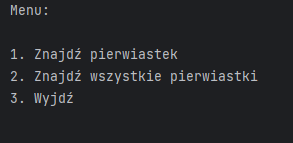
\includegraphics[width=0.5\textwidth]{menu.png}
\caption{Menu programu}
\label{fig:menu}
\end{figure}
Wybranie pierwszej opcji powoduje wyświetlenie dialogu, jak pokazano na Rys. \ref{fig:dialog}. W tym oknie należy podać niezbędne dane. Po wprowadzeniu tych wartości i~naciśnięciu klawisza Enter, program oblicza pierwiastki równania i~wyświetla je na ekranie.
\begin{figure}[H]
\centering
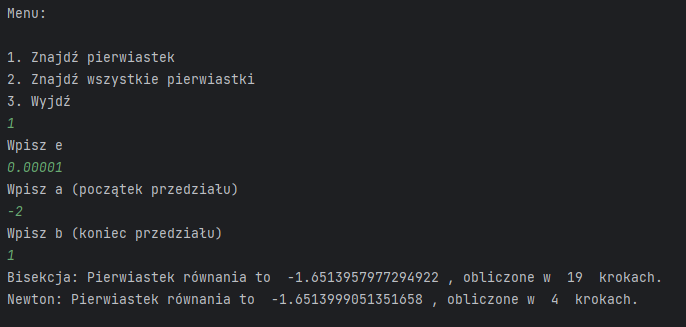
\includegraphics[width=0.8\textwidth]{menu1.png}
\caption{Dialog po wybraniu opcji 1.}
\label{fig:dialog}
\end{figure}
Po wybraniu opcji 2. program wykorzystuje metody siecznych Newtona i~bisekcji, aby obliczyć wszystkie pierwiastki danego równania. Wyniki obliczeń są wyświetlane na ekranie, jak pokazano na Rys. \ref{fig:metody}.
\begin{figure}[H]
\centering
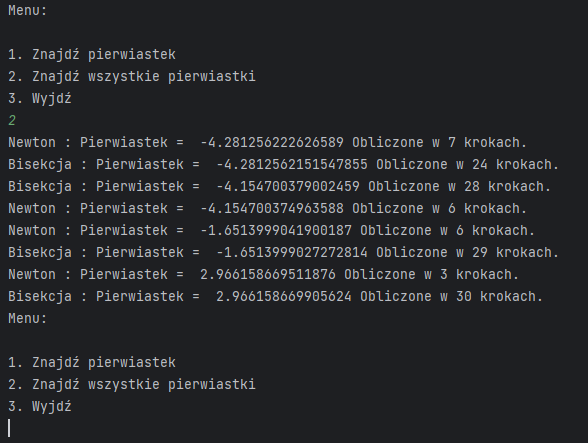
\includegraphics[width=0.8\textwidth]{menu2.png}
\caption{Obliczenie wszystkich pierwiastków równania}
\label{fig:metody}
\end{figure}
Jak można zauważyć, czasem metoda siecznych Newtona nie zbiega do rozwiązania i wtedy wyświetlony zostaje tylko jeden wynik, dla metody bisekcji.
\begin{figure}[H]
  \centering
  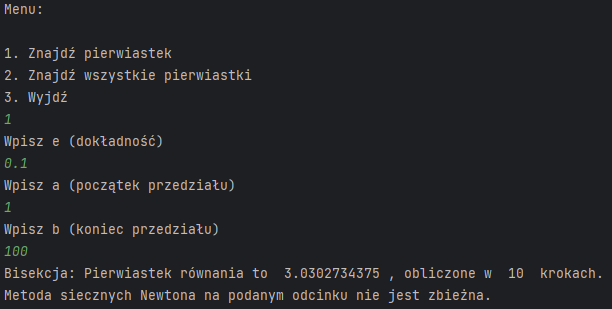
\includegraphics[width=0.8\textwidth]{1wynik.png}
  \caption{Niezbieżność metody siecznych}
\end{figure}
Wybranie opcji 3. w menu skutkuje wyjściem z programu i zakonczeniem jego działania.
\begin{figure}[H]
  \centering
  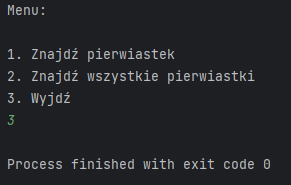
\includegraphics[width=0.5\textwidth]{menu3.png}
  \caption{Wyjście}
\end{figure}
\section{Wnioski}
Metoda siecznych Newtona jest zwykle bardziej efektywna niż metoda bisekcji, ponieważ wymaga mniejszej liczby iteracji, aby uzyskać dokładne rozwiązanie. Szybciej zbiega do rozwiązania niż metoda bisekcji.

Metoda bisekcji jest bardziej niezawodna i zapewnia zbieżność do rozwiązania, jeśli tylko funkcja jest ciągła i zmienia znak w danym przedziale. Metoda siecznych Newtona może mieć problemy ze zbieżnością, jeśli zaczynamy od złego punktu startowego. W takim przypadku metoda Newtona nie zbiega do rozwiązania.
\section{Kod programu}
\subsection{bisection.py}
\begin{minted}[breaklines]{python}
from method import Method

class Bisection(Method):
    def __init__(self, key: callable, section, e: float) -> None:
        self.section = section
        self.e = e
        self.function = key
        pass

    def solution(self) -> (float, int):
        if self.section[0]==0 or self.section[1]==0:
            print("Błąd! Funkcja jest nieokreślona w punkcie 0. Proszę wybrać punkty a,b różne od 0.")
            return 0, 0
        if (self.function(self.section[0]) * self.function(self.section[1]) >= 0):
            print("Bisekcja: Błąd! f(a)*f(b)>=0. Proszę wybrać inny przedział [a,b].")
            return 0, 0
        c = 1
        step = 0
        while self.function(c) != 0 and self.section[1] - self.section[0] > self.e:
            c = (self.section[0] + self.section[1]) / 2
            if self.function(self.section[0]) * self.function(c) < 0:
                self.section[1] = c
            else:
                self.section[0] = c
            step = step + 1
        return c, step, "Bisekcja"

\end{minted}
\subsection{main.py}
\begin{minted}[breaklines]{python}
from newton import Newton
from bisection import Bisection
import math
from newton import IterationLimit

def key(x):
    return math.log(x*x, math.e) - math.sin(x) - 2

def menu():
    print("Menu:\n")
    print("1. Znajdź pierwiastek")
    print("2. Znajdź wszystkie pierwiastki")
    print("3. Wyjdź")

def findRoot():
    e = 0
    print("Wpisz e (dokładność)")
    while e==0:
        try:
            e = float(input())
        except ValueError:
            print("Nieprawidłowy znak. Podaj liczbę zmiennoprzecinkową.")
            continue
        if e<=0 or e>=1:
            print("Dokładność nie mieści się w przedziale (0;1)")
            e = 0
        if e<math.pow(10,-15):
            print("Dokładność musi być większa od 10^-15")
            e = 0
    print("Wpisz a (początek przedziału)")
    while True:
        try:
            a = float(input())
            break
        except ValueError:
            print("Nieprawidłowy znak. Podaj liczbę zmiennoprzecinkową.")
            continue
    print("Wpisz b (koniec przedziału)")
    while True:
        try:
            b = float(input())
            if b<=a:
                print("b musi być większe od a!")
                continue
            break
        except ValueError:
            print("Nieprawidłowy znak. Podaj liczbę zmiennoprzecinkową.")
            continue
    bisect = Bisection(key, [a, b], e)
    answer = bisect.solution()
    if answer[1]>0:
        print("Bisekcja: Pierwiastek równania to ", answer[0], ",obliczone w ", answer[1], " krokach.")
    try:
        newton = Newton(key,a,b,e)
        answer2 = newton.solution()
        print("Newton: Pierwiastek równania to ", answer2[0], ",obliczone w ", answer2[1], " krokach.")
        if answer2[0]-answer[0]>e and answer[1]>0:
            print("Uwaga, prawdopodobnie na przedziale [",a,",",b,"] znajduje sie więcej niż jeden punkt zerowy funkcji.")
    except IterationLimit:
        pass

def findAllRoots(a,b,precision):
    c = b
    answers = []
    while c>=a:
        c -= precision
        if key(b)*key(c)<0:
            bisect = Bisection(key,[c,b],math.pow(10,-8))
            answer = bisect.solution()
            answers.append(answer)
            try:
                newton = Newton(key, b, c, math.pow(10,-8))
                answer = newton.solution()
                answers.append(answer)
            except IterationLimit:
                pass
            b = c
    answers = sorted(answers, key=lambda x: x[0], reverse=False)
    for x in answers:
        print(x[2],": Pierwiastek = ",x[0],"Obliczone w",x[1],"krokach.")

def main():
    cont = True
    while cont:
        menu()
        try:
            choice = int(input())
        except ValueError:
            print("Nieprawidłowy znak. Podaj liczbę 1, 2 lub 3.")
            continue
        if choice == 1:
            findRoot()
        elif choice == 2:
            findAllRoots(-10, 10, 0.001)
        elif choice == 3:
            cont = False
        else:
            print("Nieprawidłowa wartość. Podaj liczbę 1, 2 lub 3.")

if __name__ == "__main__":
    main()
\end{minted}
\subsection{method.py}
\begin{minted}[breaklines]{python}
from abc import ABC, abstractmethod

class Method(ABC):
    @abstractmethod
    def solution(self):
        pass
\end{minted}
\subsection{newton.py}
\begin{minted}[breaklines]{python}
from method import Method

class IterationLimit(Exception):
    pass

class BadInterval(Exception):
    pass

class Newton(Method):
    def __init__(self, key: callable, x_1: float, x_2: float, e: float, max_step: int = 45) -> None:
        self.key = key
        self.e = e
        self.x_1 = x_1
        self.x_2 = x_2
        self.max_steps = max_step

    def solution(self) -> (float, int):
        steps = 0
        while not self._check_diff(self.x_2, self.x_1):
            if steps > self.max_steps:
                print("Metoda siecznych Newtona na podanym odcinku nie jest zbieżna.")
                raise IterationLimit
            try:
                tmp = self._calc_next_x(self.x_1, self.x_2)
            except ZeroDivisionError:
                raise BadInterval
            self.x_1 = self.x_2
            self.x_2 = tmp
            steps += 1
        return self.x_2, steps, "Newton"

    def _calc_next_x(self, x_prev: float, x: float) -> float:
        if x==0 or x_prev ==0:
            raise IterationLimit
        return x - ((self.key(x) * (x-x_prev)) / (self.key(x) - self.key(x_prev)))

    def _check_diff(self, x, x_prev):
        self.diff = abs(x-x_prev)
        return self.diff < self.e

    def __str__(self):
        return 'Newton'
\end{minted}
\section*{Bibliografia}
\begin{thebibliography}{}
	
\bibitem{Jaruszewska-Walczak}
Jaruszewska-Walczak, D. Wykład z Algorytmów numerycznych.

\bibitem{Kincaid}
Kincaid, D., \& Cheney, W. \emph{Analiza numeryczna}.

\bibitem{Tatjewski}
Tatjewski, P. \emph{Metody numeryczne}
	
\end{thebibliography}
\end{document}
